\documentclass[twocolumn, 11pt]{article}
\usepackage[margin=0.7in]{geometry}
\usepackage{booktabs}
\usepackage{multirow}
\usepackage{graphicx}
\usepackage{paralist}
\usepackage{subcaption}

\setlength{\columnsep}{0.3in}

\makeatletter
\renewcommand{\paragraph}{%
  \@startsection{paragraph}{4}%
  {\z@}{1.25ex \@plus 1ex \@minus .2ex}{-1em}%
  {\normalfont\normalsize\bfseries}%
}
\makeatother

\title{CS224S Assignment 4}
\author{Milind Ganjoo\\\texttt{mganjoo@cs.stanford.edu}
\and%
Stephanie Lynne Pancoast\\\texttt{pancoast@stanford.edu}
\and%
Sebastian Schuster\\\texttt{sebschu@stanford.edu}}
\date{}

\begin{document}

\maketitle

\section{Classifier}

We experimented with different loss functions and regularization 
parameters using LIBLINEAR.  By default, LIBLINEAR uses a $L_2$-regularized 
$L_2$-loss SVM classification algorithm. However, $L_1$ regularization often performs better 
on  data sets with a large number of features of which several are assumed to contain little to no information
as it is able to automatically assign 0 weights to irrelevant features.
Our data set potentially contains features that contain alms no discriminatory information, 
therefore we also tried the following two classification algorithms: \begin{inparaenum}[1)] 
\item a $L_1$ regularized $L_2$ SVM classifier, and \item a $L_1$ regularized 
logistic regression classifier. \end{inparaenum} Further, we experimented with normalizing the feature
values using the following transformation for each feature value $f_i$:
$$f_i' =  \frac{f_i - \mu_i}{\sigma_i}.$$ 

\begin{table}[b]\centering
  \begin{tabular}{lcc}
    \toprule
    Classifier & Raw  & Normalized \\
    \midrule
    SVM w/ $L_2$-reg & 0.30 & 0.49 \\
    SVM w/ $L_1$-reg & 0.44 & 0.53 \\
    LogReg w/ $L_1$-reg & 0.53 & 0.52  \\
    \bottomrule
  \end{tabular}
  \caption{Accuracy for different classifiers using raw and normalized features. For all experiments we used a regularization strength $C=1$.}\label{tab:results}
\end{table}


The results are presented in Table~\ref{tab:results}. This table shows that using $L_1$ 
regularization significantly improves the classification accuracy. Using 
normalized features further improves classification accuracy 
(with the exception of logistic regression where we see a very small drop in accuracy). 

Finally, we also tried different values for the regularization strength $C$. Figure~\ref{fig:reg_strength} shows
the influence of this parameter for the three classifiers. 
Combining all these findings, we obtained the best results (an accuracy of 62\%)
using a the logistic regression classifier with normalized features and an inverse regularization
strength of $C=0.09$.

\begin{figure}[h]\centering
    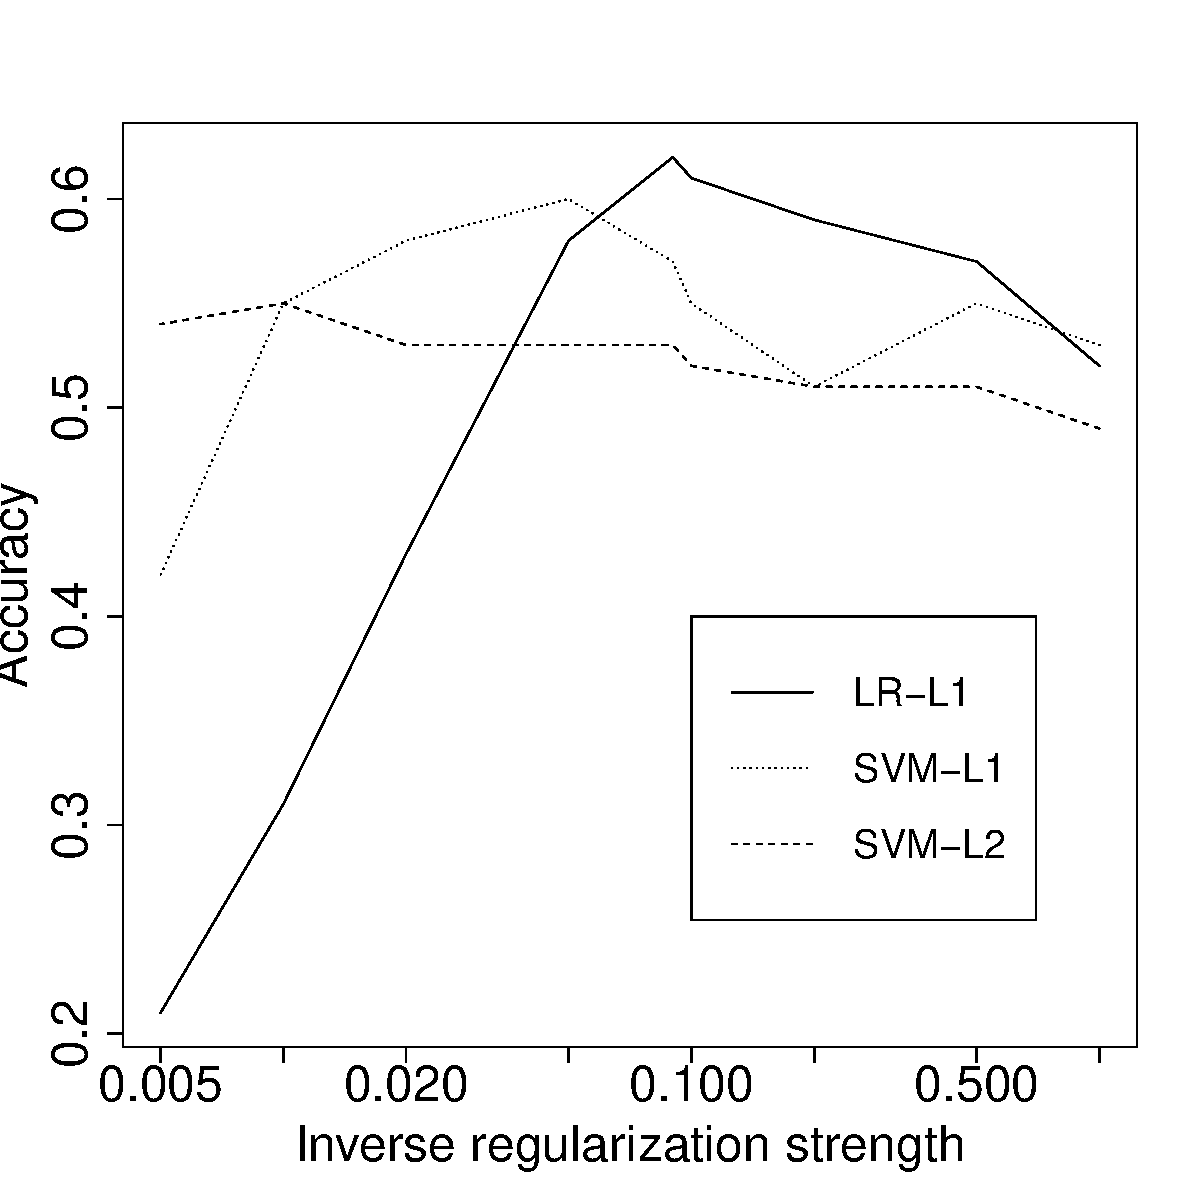
\includegraphics[width=0.7\columnwidth]{reg_strength.pdf}
    \caption{\label{fig:reg_strength} Accuracy for different classifiers with different regularization strengths. All experiments
    were conducted using normalized features.}
\end{figure}

\section{Feature Analysis}
The logistic regression classifier we used outputs weights for all of the features. Because we used a L1-loss function, many of these are zeros. More specifically, out of the 384 possible features, only 58, 65, 63, 42, and 63 were used for anger, despair, happy, neutral, and sadness, respectively. 186 of the features were given a zero weight for all five emotions. Also, no features were used for all five emotions. Only three features (MFCC3-skewness, MFCC6-max, and MFCC8-amean) were weighted non-zero for four of the five. We examined, for each emotion, the five strongest (in terms of magnitude weights) to gain insight into which features are indicative of each emotion.

\paragraph{Anger} Three of the five heaviest weighted features for anger classification are related to the MFCCs  (MFCC2-amean,  MFCC4-minPos, MFCC6-max). These are all lower to mid coefficients, indicating basic functionals of the vocal tract characterize angry speech. The other two features: F0-amean delta and energy-min are not surprising. It is expected that energy will impact the classification of anger as anger is usually associated with loud more intense speech. The changing of the F0 arithmetic mean over windows captures a feature of the pitch contour.
\paragraph{Despair} Three of the five of the top heaviest weighted feature for the despair training are related to the MFCCs delta functionals. The model learns heavy weights for MFCC3-kurtosis delta,  MFCC1-stddev delta, and MFCC10-stddev delta. This suggests that the changing of both the vocal tract and the glottal excititation are correlated with despair. Energy-maxPos also is heavily weighted with despair, indicating that when we act despairingly, we adjust where in an utterance we place the most energy. The final feature, voiceprob-delta kurtosis indicates the amount of voicing in depair utterances is somehow correlated with the emotion.
\paragraph{Happy} All five of the top features for the happy utterances involve MFCCs. MFCC1-range, MFCC6-max, MFCC7-amean, MFCC9-linregerrQ and MFCC12-amean receive the top five weights (thought not listed in order of rank here). This suggests that the basic characteristics of our vocal tract behavior and our average glottal excitation correlated with what we consider "happy". 
\paragraph{Neutral} For neutral speech, the top five features were again all related to MFCCs. MFCC1-amean, MFCC1-linregerrQ delta, MFCC2-max, MFCC4-delta skewness, MFCC8-linrecg2. There is a lack of influence from the higher coefficients, which remains true when examing the top ten weighted features (which are all still derived from MFCC 1 through 8), indicating glottal excitation does not correlate with neutral versus emotional speech.
\paragraph{Sadness} The heaviest weighted feature for sadness is the min energy. This is very expected, as we as humans associate sadness with less energy. The other top-four features include MFCC2-kurtosis delta, MFCC8-linregerrQ, MFCC4-skewness delta, and MFCC7-linregerrQ. 

\section{Error Analysis}
We generated a confusion matrix for the emotion classifications which is included in the table below. As is consistent with the literature, we observe that neutral speech is the easiest to classify and also the most frequently recipient of a mis-classification. Sadness is misclassified as neutral 9 times, the most of any misclassification pair in our test set. This is not so suprising as neutral and sadness use similarly features in their classifiers. Despair segments are only correctly classified $40\%$ of the time, making the emotion the most difficult to identify. 

\begin{table}[tbp]
\centering
\begin{tabular}{|c|c|c|c|c|c|}
\hline
&A & D & H & N & S  \\
\hline
Anger (A) & \bf 29 & 1 & 4 & 0 & 2 \\
Despair (D) & 1 & \bf 14 & 7 & 5 & 8 \\
Happiness (H) & 3 & 8 & \bf 18 & 4 & 2\\
Neutral (N) & 0 & 0 & 0 & \bf 23 & 2\\
Sadness (S) & 0 & 5 & 2 & 9 & \bf 18\\
\hline
\end{tabular}
\caption{\footnotesize Confusion matrix for emotion classification.}
\end{table}



\end{document}
